\documentclass[12pt,preprint]{aastex}

% has to be before amssymb it seems
\usepackage{color,hyperref}
\definecolor{linkcolor}{rgb}{0,0,0.5}
\hypersetup{colorlinks=true,linkcolor=linkcolor,citecolor=linkcolor,
            filecolor=linkcolor,urlcolor=linkcolor}

\usepackage{url}
\usepackage{algorithmic,algorithm}
\usepackage{amssymb,amsmath}
\usepackage{graphicx}
\graphicspath{{figures/}}

\newcommand{\arxiv}[1]{\href{http://arxiv.org/abs/#1}{arXiv:#1}}

\usepackage{listings}
\definecolor{lbcolor}{rgb}{0.9,0.9,0.9}
\lstset{language=Python,
        basicstyle=\footnotesize\ttfamily,
        showspaces=false,
        showstringspaces=false,
        tabsize=2,
        breaklines=false,
        breakatwhitespace=true,
        identifierstyle=\ttfamily,
        keywordstyle=\bfseries\color[rgb]{0.133,0.545,0.133},
        commentstyle=\color[rgb]{0.133,0.545,0.133},
        stringstyle=\color[rgb]{0.627,0.126,0.941},
    }

\newcommand{\project}[1]{{\sffamily #1}}
\newcommand{\Python}{\project{Python}}
\newcommand{\numpy}{\project{numpy}}
\newcommand{\Ubuntu}{\project{Ubuntu}}
\newcommand{\github}{\project{GitHub}}
\newcommand{\pip}{\project{pip}}
\newcommand{\acor}{\project{acor}}
\newcommand{\thisplain}{emcee}
\newcommand{\this}{\project{\thisplain}}
\newcommand{\paper}{document}
\newcommand{\license}{MIT License}

\newcommand{\foreign}[1]{\emph{#1}}
\newcommand{\etal}{\foreign{et\,al.}}
\newcommand{\etc}{\foreign{etc.}}

\newcommand{\Fig}[1]{Figure~\ref{fig:#1}}
\newcommand{\fig}[1]{\Fig{#1}}
\newcommand{\figlabel}[1]{\label{fig:#1}}
\newcommand{\Tab}[1]{Table~\ref{tab:#1}}
\newcommand{\tab}[1]{\Tab{#1}}
\newcommand{\tablabel}[1]{\label{tab:#1}}
\newcommand{\Eq}[1]{Equation~(\ref{eq:#1})}
\newcommand{\eq}[1]{\Eq{#1}}
\newcommand{\eqlabel}[1]{\label{eq:#1}}
\newcommand{\Sect}[1]{Section~\ref{sect:#1}}
\newcommand{\sect}[1]{\Sect{#1}}
\newcommand{\App}[1]{Appendix~\ref{sect:#1}}
\newcommand{\app}[1]{\App{#1}}
\newcommand{\sectlabel}[1]{\label{sect:#1}}
\newcommand{\Algo}[1]{Algorithm~\ref{algo:#1}}
\newcommand{\algo}[1]{\Algo{#1}}
\newcommand{\algolabel}[1]{\label{algo:#1}}

% math symbols
\newcommand{\dd}{\mathrm{d}}
\newcommand{\like}{\mathscr{L}}
\newcommand{\bvec}[1]{\boldsymbol{#1}}
\newcommand{\paramvector}[1]{\bvec{#1}}
\newcommand{\normal}[2]{\mathcal{N} (#1, #2)}
\newcommand{\ensemble}{S}
\newcommand{\colorens}[1]{\ensemble^{(#1)}}
\newcommand{\red}{\colorens{0}}
\newcommand{\blue}{\colorens{1}}
\renewcommand{\vector}[1]{#1}
\renewcommand{\matrix}[1]{#1}
\newcommand{\pr}[1]{\ensuremath{p(#1)}}
\newcommand{\af}{\ensuremath{a_f}}
\newcommand{\expect}[1]{\left<#1\right>}

% model parameters
\newcommand{\model}{\ensuremath{\vector{\Theta}}}
\newcommand{\data}{\ensuremath{\vector{D}}}
\newcommand{\nuisance}{\ensuremath{\vector{\alpha}}}
\newcommand{\link}{\ensuremath{X}}

% units
\newcommand{\unit}[1]{\mathrm{#1}}

\begin{document}

\title{Multiband Periodograms of Astronomical Sources}

\newcommand{\escience}{1}
\newcommand{\uwastro}{2}
\author{Jacob T. VanderPlas\altaffilmark{\escience}}
\author{{\v Z}eljko Ivezi{\'c}\altaffilmark{\uwastro}}
\altaffiltext{\escience}{eScience Institute, University of Washington}
\altaffiltext{\uwastro}{Department of Astronomy, University of Washington}


\begin{abstract}
  This paper introduces a general method for least-squares spectral fitting of multi-band periodic data.
\end{abstract}

\keywords{
    methods: data analysis ---
    methods: numerical ---
    methods: statistical
}

\section{Introduction}

\begin{itemize}
  \item Lomb Scargle periodograms \& their use in Astronomy
  \item Other methods of period finding (Supersmoother, ARMA-type models, etc.)
  \item Need for multi-band periodograms
\end{itemize}

\section{Multiterm Periodograms: Background}

\begin{itemize}
  \item Relationship between Fourier Periodogram \& Least Squares fit \citep{Jaynes96}
  \item Matrix form of linear models
  \item Generalization of single-term to multi-term models
  \item Show expression for Power; refer to appendix for computational details
\end{itemize}

\section{Moving to Multiple Bands}

\begin{itemize}
  \item Write-out the linear model
  \item Demonstrate the matrix form of this
  \item Use light regularization
  \item Correspondance of the single-term multiband result to the weighted sum of single-band Lomb-Scargle results
\end{itemize}

\section{Examples}
\subsection{Simulated Example}

\begin{figure}
  \centering
  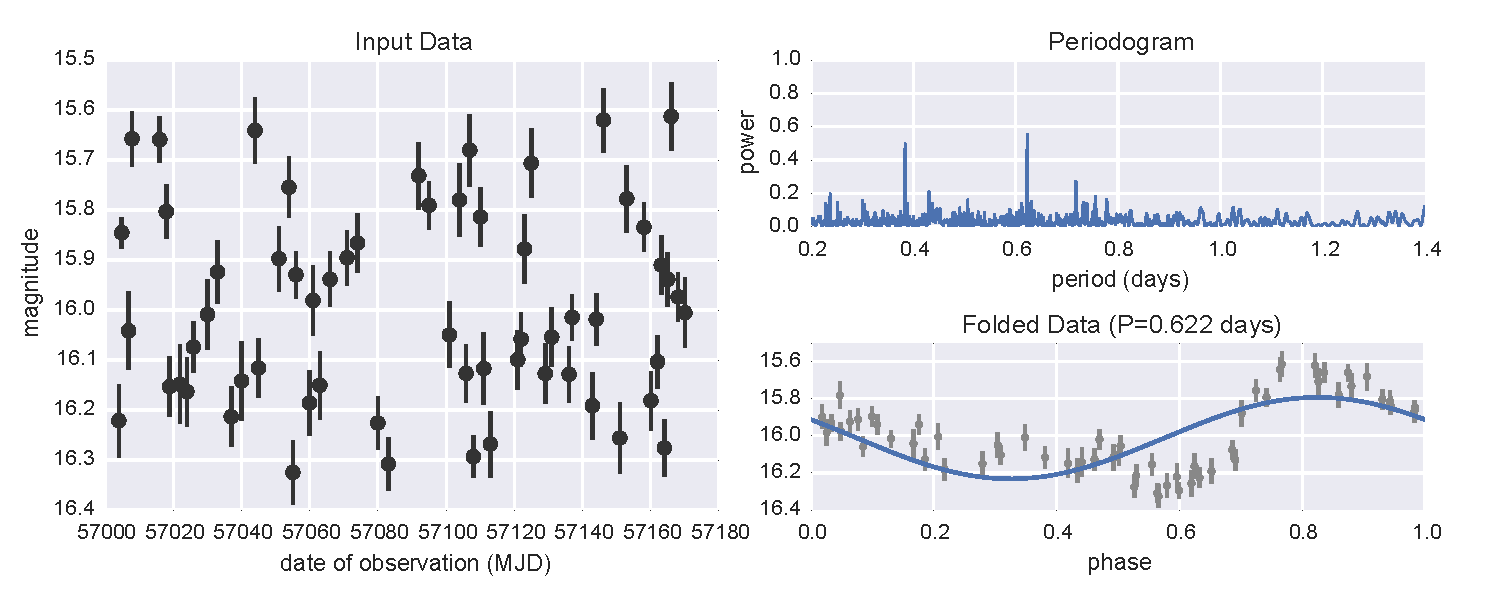
\includegraphics[width=\textwidth]{fig01.pdf}
  \caption{
    An illustration of the typical approach to multiband periodograms,
    in which each band is fit individually. The data consists of 60 coeval
    u-g-r-i-z observations spread over 180 nights, and is based on an
    RR Lyrae template from \citet{Sesar2010}. With this much data in each
    band, individual periodograms can be constructed and compared to find the
    true period $P=0.622$ days.
  }
  \label{fig:01}
\end{figure}

\begin{figure}
  \centering
  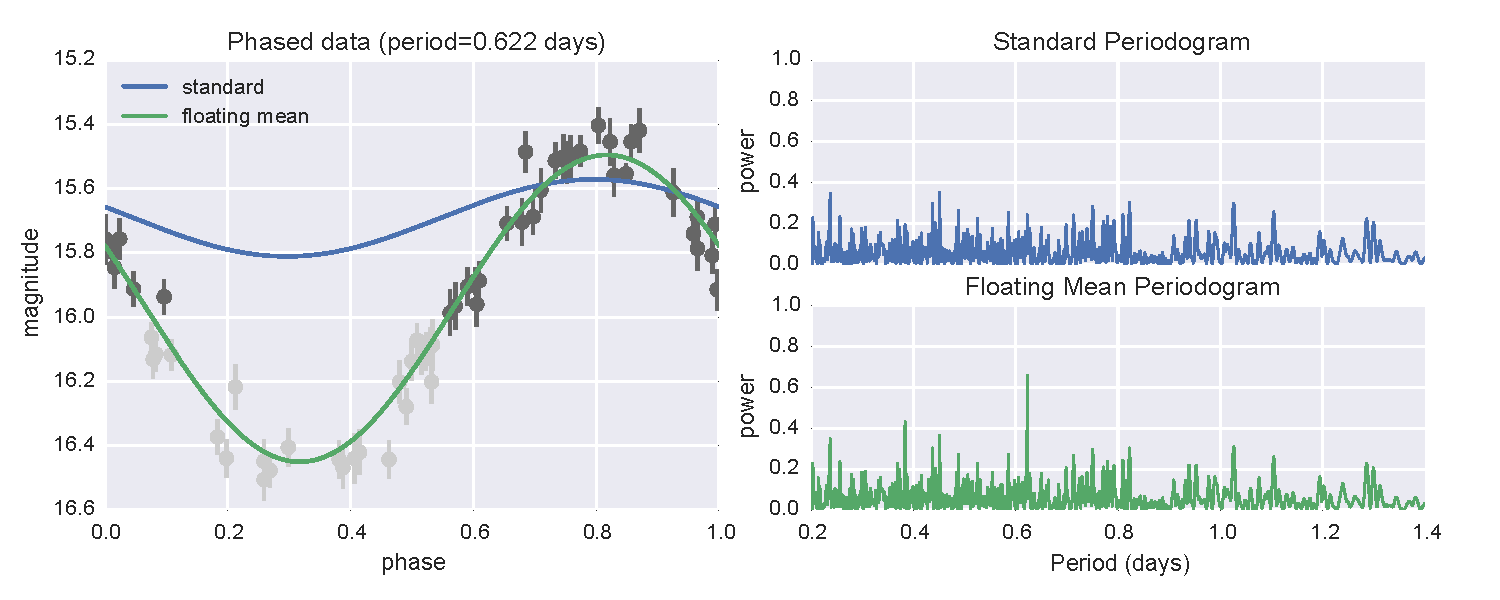
\includegraphics[width=\textwidth]{fig02.pdf}
  \caption{
    Another realization of the data from \fig{01}, with only a single-band
    observation each night (i.e. 12 observations per band, spread over 180
    days). In this case, there is not enough data in each band to recover
    periodicity information. By applying the multiband approach which utilizes
    all the data at once (lower right), we again see a significant spike of
    power at the true period $P=0.622$ days.    
  } 
  \label{fig:02}
\end{figure}

\begin{itemize}
  \item Show power spectrum for a single-band RR-Lyrae
  \item Reduce observations, show multiple power spectra for multi-band RR-Lyrae
  \item Show single power spectrum for multi-band RR-Lyrae
\end{itemize}

\subsection{Stripe 82}

\begin{itemize}
  \item Compute periods using majority method
  \item Compute periods using unified method
  \item Compare the results
\end{itemize}

\section{Further work}

\begin{itemize}
  \item issues with window function corrections
  \item issues with physicality of model
\end{itemize}


\bibliographystyle{apj}
\bibliography{paper}


\appendix


\section{The Lomb-Scargle Periodogram and Least-Squares Spectral Fitting}

We start with time-series data

\begin{equation}
  D = \{t_i,y_i,\sigma_i\}_{i=1}^N
\end{equation}

without loss of generality, we will assume throughout that the $y_i$ values are centered; that is, the weighted mean

\begin{equation}
  \label{eq:centered-data}
  \frac{\sum_{i=1}^N w_i y_i}{\sum_{i=1}^N w_i} = 0
\end{equation}

where the weights are $w_i \equiv \sigma_i^{-2}$. We will seek a single sinusoid model which fits this data; that is, our model is

\begin{equation}
M(t~|~A,\omega,\phi) = A \sin(\omega t + \phi)
\end{equation}

to make this a linear problem,

\begin{equation}
M(t~|~\omega,\theta) = \theta_0 \sin(\omega t) + \theta_1\cos(\omega t)
\end{equation}

which can be related to the above form by $\theta_0 = A\cos\phi$ and $\theta_1 = A\sin\phi$.
The $\chi^2$ for this model is given by

\begin{equation}
\chi^2(D, \omega, \theta) = \sum_i\frac{[y_i - M(t_i~|~\omega,\theta)]^2}{2\sigma_i^2}
\end{equation}

This can be expressed more compactly by defining the following matrices:

\begin{equation}
X_\omega = \left[
\begin{array}{cc}
\sin(\omega t_1) & \cos(\omega t_1)\\
\sin(\omega t_2) & \cos(\omega t_2)\\
\vdots & \vdots \\
\sin(\omega t_N) & \cos(\omega t_N)\\
\end{array}
\right];~~
y = \left[
\begin{array}{c}
y_1 \\
y_2\\
\vdots \\
y_N\\
\end{array}
\right];~~
\Sigma = \left[
\begin{array}{ccccc}
\sigma_1^2 & 0 & 0 & \cdots & 0\\
0 & \sigma_2^2 & 0 & \cdots & 0\\
0 & 0 & \sigma_3^2 & \cdots & 0\\
\vdots & \vdots & \vdots & \ddots & \vdots\\
0 & 0 & 0 & \cdots & \sigma_N^2
\end{array}
\right]
\end{equation}

Then the model is given by $X_\omega\theta$ and the $\chi^2$ can be written
compactly as:

\begin{equation}
  \chi^2(\omega, \theta) = (y - X_\omega\theta)^T\Sigma^{-1}(y - X_\omega\theta)
\end{equation}

Minimizing this cost funciton with respect to $\theta$ gives the maximum likelihood parameters:

\begin{equation}
\hat{\theta}_\omega = (X_\omega^T\Sigma^{-1}X_\omega)^{-1}X_\omega^T\Sigma^{-1}y
\end{equation}

We'll simplify this slightly by defining the quantities $\tilde{X}_\omega = \Sigma^{-1/2}X_\omega$ and $\tilde{y} = \Sigma^{-1/2}y$, so that the maximum likelihood parameters can be written

\begin{equation}
  \hat{\theta}_\omega = (\tilde{X}_\omega^T\tilde{X}_\omega)^{-1}\tilde{X}_\omega^T\tilde{y}
\end{equation}

Now the value of $\chi^2$ at maximum likelihood can be expressed:

\begin{equation}
  \chi^2(\omega, \hat{\theta}_\omega) = \tilde{y}^T\tilde{y} - \tilde{y}^T\tilde{X}_\omega(\tilde{X}_\omega^T\tilde{X}_\omega)^{-1}\tilde{X}_\omega^T \tilde{y}
\end{equation}

The form of this equation suggests defining a reference $\chi^2$ value which is given by a best-fit constant model to the data: because of the constraint given in Eqn.~\ref{eq:centered-data}, this reference is simply written $\chi^2_0 = \tilde{y}^T\tilde{y}$. We can now follow Lomb [ref] \& Scargle [ref] and write the normalized periodogram:

\begin{eqnarray}
  \label{eq:power}
  P(\omega) &\equiv& 1 -\frac{\chi^2(\omega, \hat{\theta}_\omega)}{\chi^2_0(\omega)}\\ &=& \frac{\tilde{y}^T\tilde{X}_\omega(\tilde{X}_\omega^T\tilde{X}_\omega)^{-1}\tilde{X}_\omega^T \tilde{y}}{\tilde{y}^T\tilde{y}}
\end{eqnarray}

Typically, the Lomb-Scargle periodogram is expressed in terms of various weighted sums of sines and cosines of the data; this expression is equivalent, but has the advantage that it can be trivially generalized to an arbitrary linear model through adding columns to the $X$ matrix, and can handle arbitrary correlated measurement errors by adding appropriate off-diagonal terms to the $\Sigma$ matrix.

\section{Higher-order Models}

As an example of one of these generalizations, consider the {\it generalized Lomb-Scargle} method of \citep{Zechmeister09}. This adjusts the classic Lomb-Scargle algorithm by using a model with a floating mean, which can be more accurate for certain observing cadences:

\begin{equation}
  M(t~|~\omega, \theta) = \theta_0 + \theta_1\sin\omega t + \theta_2\cos\omega t
\end{equation}

The normalized power under this model can be computed by simply adding a column of ones to the $X$ matrix.

In a similar vein, the power for a truncated Fourier series model of any order can be constructed by extending the $X$ matrix with appropriate columns; for example, for a 2-term truncated Fourier fit with a floating mean we can write

\begin{equation}
X_\omega = \left[
\begin{array}{ccccc}
1 & \sin(\omega t_1) & \cos(\omega t_1) & \sin(2\omega t_1) & \cos(2\omega t_1)\\
1 & \sin(\omega t_2) & \cos(\omega t_2) & \sin(2\omega t_2) & \cos(2\omega t_2)\\
1 & \sin(\omega t_3) & \cos(\omega t_3) & \sin(2\omega t_3) & \cos(2\omega t_3)\\
\vdots & \vdots & \vdots & \vdots & \vdots \\
1 & \sin(\omega t_N) & \cos(\omega t_N) & \sin(2\omega t_N) & \cos(2\omega t_N)\\
\end{array}
\right]
\end{equation}

Plugging this $X$ matrix into Eqn.~\ref{eq:power} will give us the normalized periodogram associated with the two-term truncated Fourier model.

\section{Regularized Models}

(Show how regularization works its way through the equations \& derive expression for power).


\end{document}
